\documentclass[landscape,paperwidth=43truein,paperheight=33.1truein,fontscale=0.3]{baposter}
\usepackage{graphics}
\usepackage{color}
\usepackage{multicol}
\usepackage{amsmath}
\usepackage{amssymb, wasysym}
\usepackage{lipsum}
\usepackage{graphicx}

\begin{document}
\definecolor{myfavoritecolor}{rgb}{0.0 2.55 0}

%:Background image
\background{
      \begin{tikzpicture}[remember picture,overlay]%
      \draw (current page.center)+(-0em,-10em) node[anchor=center]
      {\includegraphics[width=1.2\textwidth]{images/teal_sun}};
      \end{tikzpicture}%
      }

\begin{poster}
{%Keyword=value pairs
  % Color style
background = user,
 bgColorOne=white,
  bgColorTwo=red,
  borderColor=black,
  headerColorOne=black,
  headerColorTwo=gray,
  headerFontColor=white,
  boxColorOne=white,
  boxColorTwo=myfavoritecolor,
  % Format of textbox
  textborder=roundedleft,
  % Format of text header
  eyecatcher=true,
  headerborder=closed,
  headerheight=0.15\textheight,
  headershape=roundedright,
  headershade=shadelr,
  boxshade=plain,
  headerfont=\Large\textrm,
}
{%Eyecatcher
   \resizebox{!}{.18\textheight}{
\includegraphics{inverted_solar_physics_logo.png}}
}
{%Poster Title
   {\color{white}Software Development for MOSES Flight Operations}
}
{%Author
  \color{white} Roy Smart, Jackson Remington, David Keltgen, Justin Hogan, Charles C.\ Kankelborg\\
   \textit{Physics Department, Montana State University, Bozeman, MT 59717}\\
   roytsmart@gmail.com\\
}
{%Logo
   \resizebox{!}{.13\textheight}{
\includegraphics{msuvertcmyk.pdf}}
}

%%%%%%%%%%%%%%%%%%%%%%%%%%%%%%%%%%%%
%         Zeroth Column            %
%%%%%%%%%%%%%%%%%%%%%%%%%%%%%%%%%%%%

\headerbox{Abstract}{name=abstract,column=0}{

 The Multi Order Solar EUV Spectrograph (MOSES) sounding rocket payload is a slitless spectrograph that allows snapshot imaging spectroscopy of the Sun in extreme ultraviolet (EUV) wavelengths
(Fox, Kankelborg and Thomas, 2010 Astrophys.J., 719:1132-1143). The MOSES payload relies on an embedded flight computer and FPGA
to control the instrument, command exposures from the cameras, save the experimental data, and send
the data with additional telemetry back to Earth. Replacing the previous command and data handling
system with a low-power solution necessitated the development of new software that could satisfy the
same requirements as last mission while improving on the latencies present in the old flight software. 
The new configuration is still in development, and is undergoing debugging and optimization in prepara
tion for launch.
The updated software accomplishes
our goal of improvement over the flight software implemented in the previous flight, lower latency between subsequent images, and being able to successfully transmit
images back to Earth.

}

\headerbox{First Launch}{name=launch,column=1}{
\begin{tabular}{ll}
   \begin{minipage}{0.75\columnwidth}
      \textit{MOSES} was 
      first launched on February 8, 2006 on a from White Sands Missile Range on a Black Brant IX sounding rocket.  The next launch will include updated optics and electronics and is scheduled for summer 2015.
   \end{minipage} &
   \begin{minipage}{0.15\columnwidth}
      \resizebox{\columnwidth}{!}{\includegraphics{images/MOSESinFlight.png}}
   \end{minipage}
\end{tabular}
}

\headerbox{Data Interface}{name=interface,column=1,span=2, below=launch}{
The new flight computer is designed as a drop-in replacement for the old flight computer, so it must interface with the instrument in the same way. The primary means of controlling the instrument are through \textbf{timers}, which are single-ended inputs configured to trigger events (e.g. data start/stop) at predefined times during flight. For redundancy, two other interfaces can also be used to control the instrument, \textbf{uplinks} and \textbf{HLP packets}.
}
\headerbox{Hardware Solutions}{name=hardware,column=3}{
The VDX104+ is the flight computer for the instrument. It provides a GNU/Linux operating system for development, ethernet and RS-232 serial ports for communication, and PCI-104 bus for interfacing with the FPGA. The flight software designed by our team runs on this device.
\begin{center}
\resizebox{.70\columnwidth}{!}{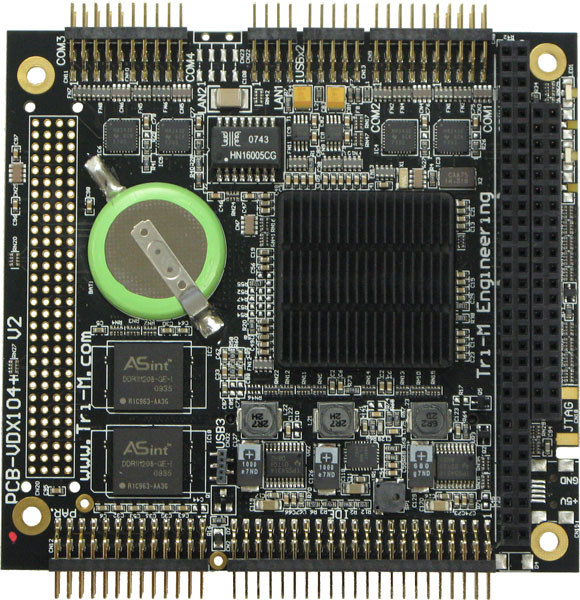
\includegraphics{images/vdx104}} \\
\footnotesize{VDX104 flight computer}
\end{center}

The Virtex5 FPGA captures the 32 Mbit/s parallel data produced by the experiment and various GPIO. It then transfers the data through DMA to the flight computer for transmitting.
\begin{center}
\resizebox{.70\columnwidth}{!}{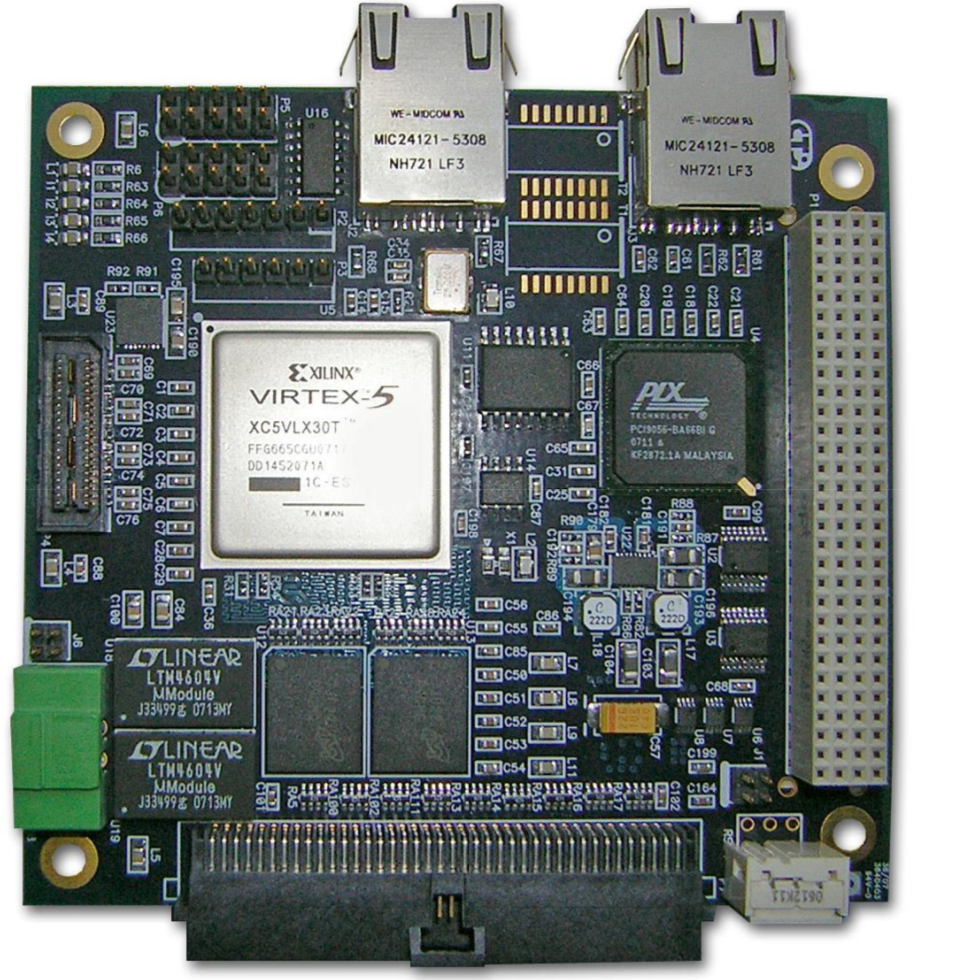
\includegraphics{images/fpga}} \\
\footnotesize{Connect Tech FreeForm PCI-104 w/ Virtex5 FPGA}
\end{center}

}

\headerbox{Software Architecture}{name=arch,column=0,span=3, below=abstract}{
\begin{tabular}{ll}
  \begin{minipage}{0.20\columnwidth}
     The flight software relies on a threaded architecture to reliably respond to a variety of inputs, all while the processor is actively capturing data. Several thread-synchronization techniques have been utilized, including mutex-protected queues, Linux Signals, and semaphores. 

  \end{minipage}&
  \begin{minipage}{0.75\columnwidth}
      \resizebox{\columnwidth}{!}{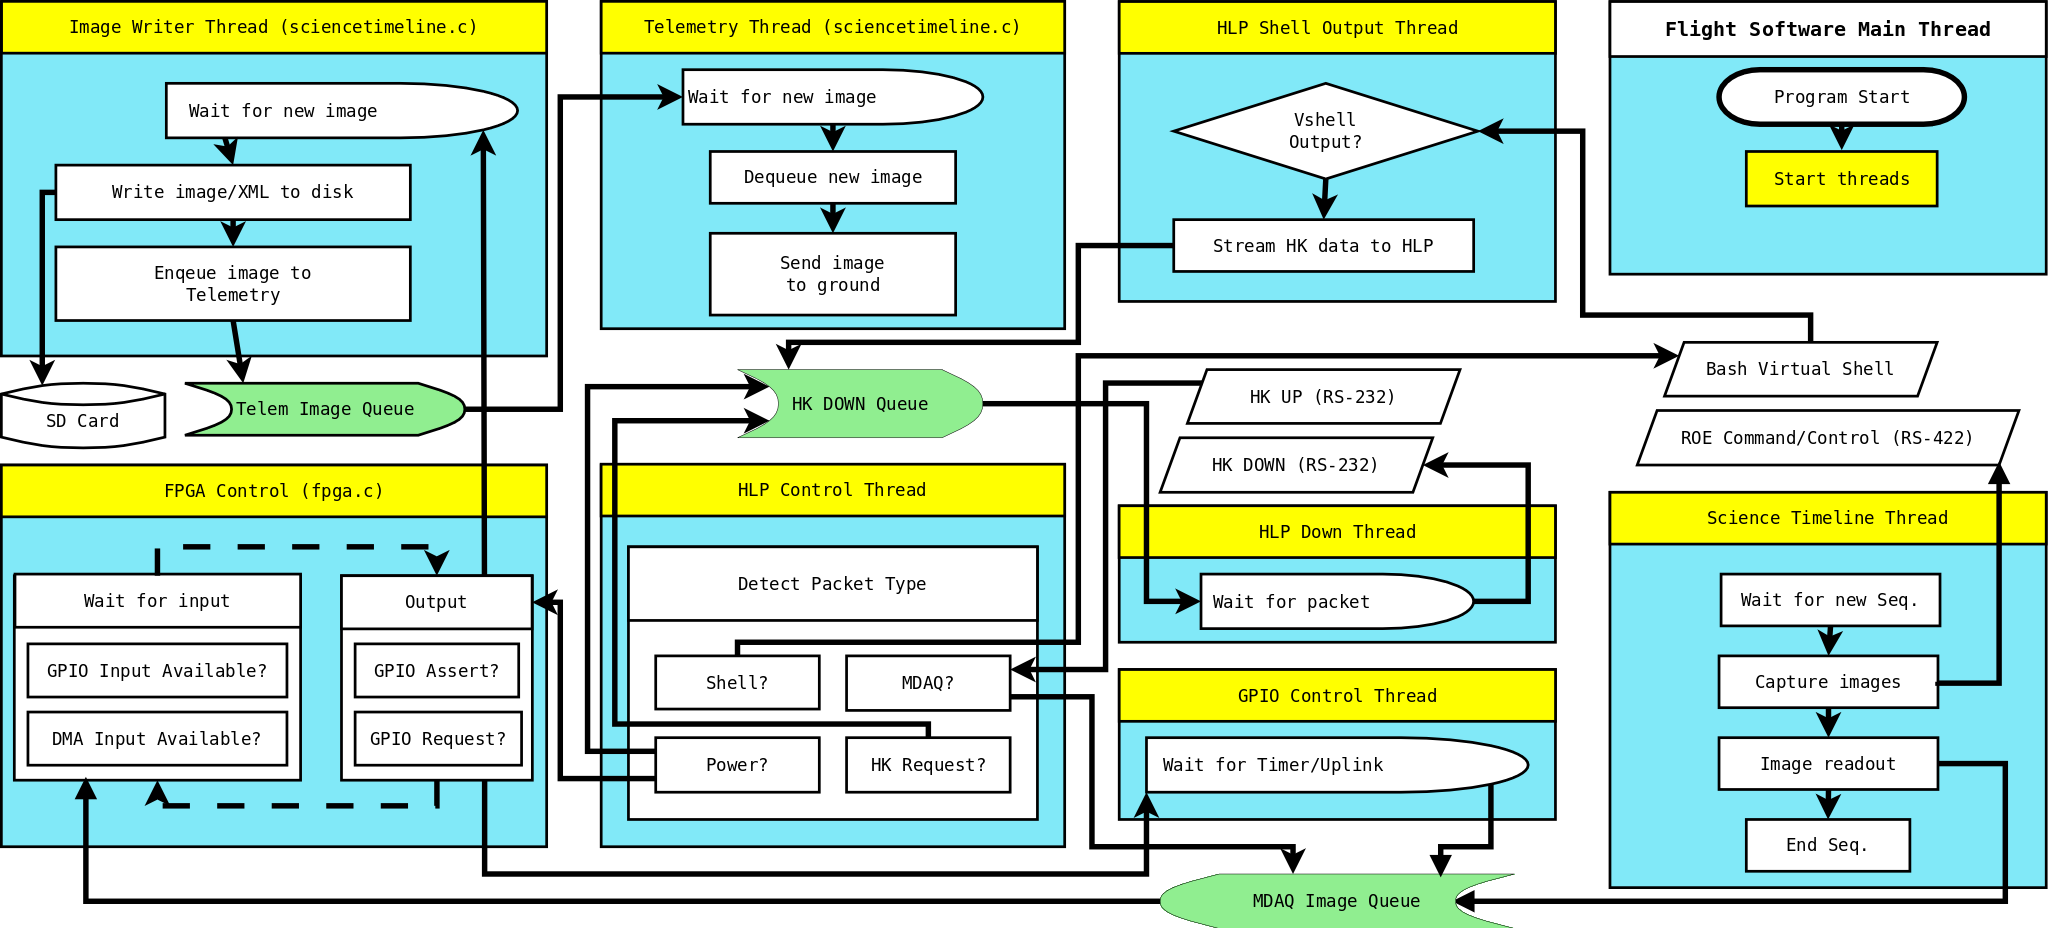
\includegraphics{images/mfsw_poster}}
      \footnotesize{HK packet on Oscilloscope}  
\end{minipage}  
\end{tabular}
}

\end{poster}

\end{document}